\section{Diseño del software} % (fold)
\label{sec:diseno_del_software}


Con la elección del microcontrolador C8051F350, se procedió a la etapa de diseño del sistema. Para ilustrar el diseño, se utilizan diagramas UML.

\subsection{Diagrama de bloques} % (fold)
\label{sub:diagrama_de_bloques}

\begin{figure}[h]
  \centering
  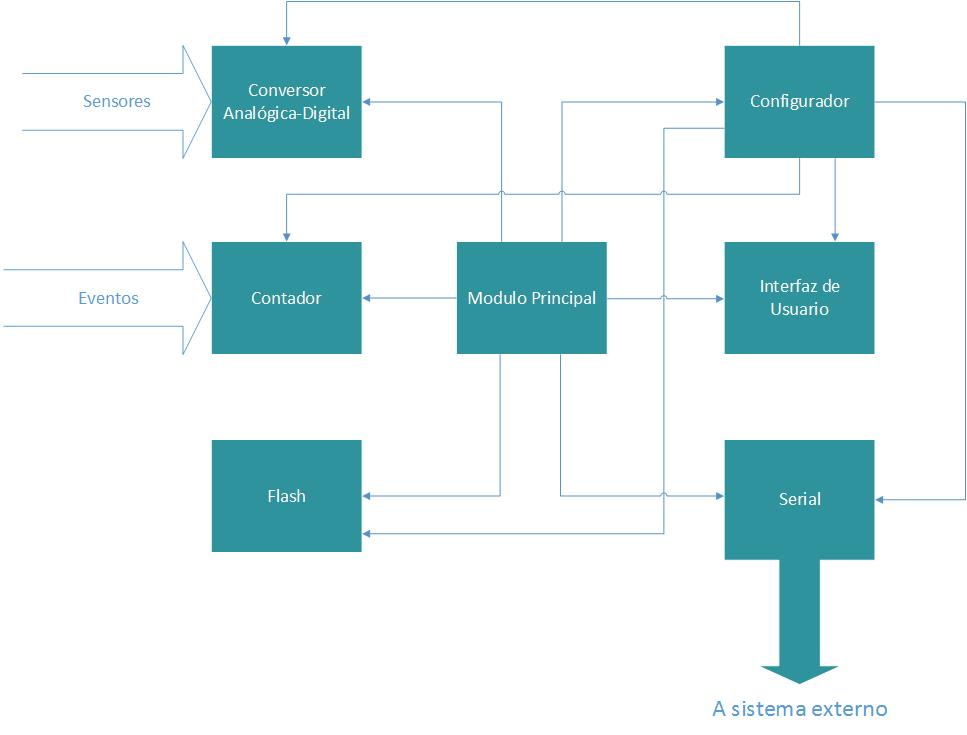
\includegraphics[width=0.80\textwidth, height = 9cm]{Bloques1}
  \caption{Diagrama de Bloques del sistema}\label{fig:bloques1}
\end{figure}

\paragraph{}
El sistema esta compuesto por 6 bloques o módulos separados, manejados por un modulo principal. En la figura \ref{fig:bloques1} se pueden observar estos bloques y la interacción que tienen entre si. 
\paragraph{}


\begin{itemize}
  \item El \textbf{Bloque Principal} se encarga ejecutar las funciones del resto de los módulos para dar arranque y ejecución al sistema.
  \item El \textbf{Bloque Conversor Analógico-Digital} principalmente obtiene los datos de los sensores, los procesa, y los envía al modulo principal. Además de esto, configura el funcionamiento del ADC según los parámetros dados por el usuario. El usuario puede elegir la cantidad de pines que va a utilizar como entrada según la cantidad de sensores que quiera medir, puede elegir un nivel de ganancia de amplificación de la señal antes de la conversión, y puede también elegir el modo de obtención de los datos (diferencial o single-ended).
  \item El \textbf{Bloque Contador} se encarga de obtener los valores en los contadores de eventos.
  \item El \textbf{Bloque de Interfaz de Usuario} levanta la interfaz con la que interactúa el usuario para establecer los parámetros configurables del sistema.
  \item El \textbf{Bloque Configurador} interactúa directamente con el hardware del microcontrolador. Realiza todas las configuraciones necesarias para poder hacer funcionar cada modulo. Es por esto que en el diagrama de bloques se puede ver que este modulo interactúa directamente con todos los demás. Inicializa todos los registros pertinentes, el clock del sistema y setea los puertos de entrada y salida.
  \item El \textbf{Bloque Serial} envía los datos por interfaz UART.
  %\item El \textbf{Bloque Flash} Maneja la unidad de memoria no volatil del sistema. Se utiliza para guardar y cargar configuraciones hechas por el usuario, de forma que puedan cargarse automaticamente al inicio del sistema sin necesidad de volver a configurarlo cada vez que se inicia.
\end{itemize}

\subsection{Mención sobre la memoria flash} % (fold)
\label{sub:mencion_sobre_la_memoria_flash}

Con respecto al informe de las 100 horas, se removió el bloque flash del diseño. En un principio, se pensó en la posibilidad de utilizar la memoria flash del microcontrolador para guardar configuraciones, de forma que no sea necesario configurar el sistema desde 0 cada vez que se inicia. Pero esto no pudo ser posible. Las operaciones necesarias para leer y escribir la memoria y el tamaño de la misma hicieron que sea difícil realizar la escritura y la lectura de la misma.

Para escribir una palabra en memoria, es necesario borrar toda la pagina en donde se encuentra la palabra para luego reescribirla. Cada pagina de la memoria flash ocupa 512 Bytes.

Tanto el programa que corre en el microprocesador como los datos de configuración debe guardarse en la misma memoria flash de 8Kb. El programa ocupa alrededor de 7Kb. En el Kb que sobra, es posible guardar las configuraciones, pero lo que lo dificulta es que el método de escritura de la flash pone en riesgo la integridad del programa. Teniendo en cuenta esto, se decidió no utilizar la flash para guardar las configuraciones. Por lo tanto, cada vez que el sistema se apague, se pierden las configuraciones, sin posibilidad de guardarlas.

% subsection mencion_sobre_la_memoria_flash (end)

\subsection{Mención sobre SMBus} % (fold)
\label{sub:mencion_sobre_smbus}

En los requerimientos, se especifica que es necesario que se puedan transmitir los datos de las mediciones utilizando protocolo UART tanto con RS232 como con $I^{2}$C. El microcontrolador cuenta con una interfaz serial$^{\tiny{\ref{sub:interfaz_serial}}}$ llamada SMBus, que puede comunicarse con cualquier dispositivo que utilice $I^{2}$C porque es compatible. Sin embargo, fue complicado lograr que funcione, y luego de hacer algunas investigaciones, se encontró que suele ser un problema común que esta interfaz no suela funcionar en estos microcontroladores. Luego de intentar reiteradas veces sin obtener resultados, se opto por no utilizar SMBus y trabajar únicamente con el protocolo UART.



% subsection mencion_sobre_smbus (end)

% subsubsection diagrama_de_bloques (end)

\subsubsection{Diagramas de caso de uso} % (fold)
\label{ssub:diagramas_de_caso_de_uso}

En la figura \ref{fig:casouso1} se muestra un diagrama de caso de uso del sistema. Los casos de uso son bastante intuitivos, el usuario debe poder configurar todos los aspectos claves del sistema. Este diagrama muestra a grandes rasgos las acciones posibles que pueden hacerse sobre el sistema desde el punto de vista del usuario.

\begin{figure}[h]
  \centering
  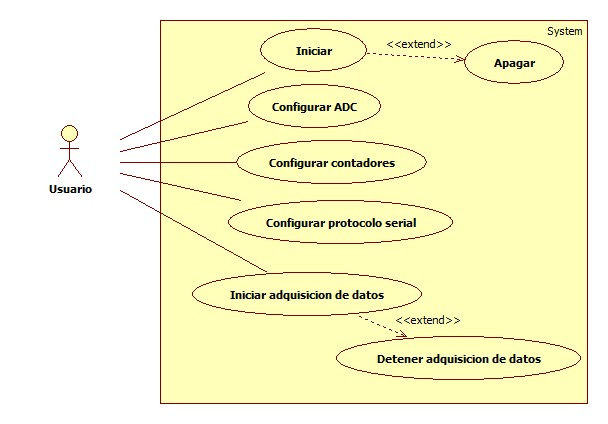
\includegraphics[width=0.80\textwidth, height = 9cm]{CasoUso1}
  \caption{Diagrama de caso de uso}\label{fig:casouso1}
\end{figure}

% subsubsection diagramas_de_caso_de_uso (end)

\subsubsection{Diagramas de secuencia} % (fold)
\label{ssub:diagramas_de_secuencia}

Los diagramas de secuencia modelan distintas interacciones entre los componentes de un sistema. En este caso, los dos componentes mas importantes del sistema son el usuario, y el programa principal que recibe las peticiones del usuario a través de la interfaz gráfica, y procesa los pedidos llamando a funciones de otros bloques del sistema. En el primer diagrama (figura \ref{fig:secuencia1}) se modelo una configuración de un pin especifico para medir una entrada analógica. El programa principal, en este caso, debe llamar a funciones del bloque conversor para configurar el pedido del usuario. Luego, el usuario habilita el comienzo de conversión para que el sistema envié los datos ya digitales por interfaz serial.


\begin{figure}[h]
  \centering
  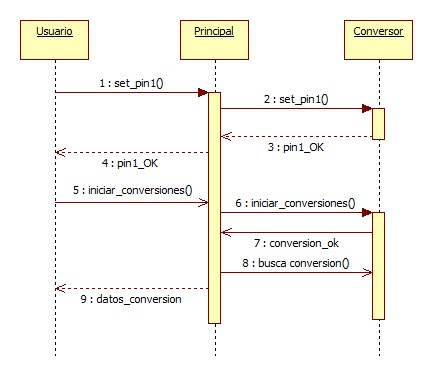
\includegraphics[width=0.50\textwidth, height = 7cm]{Secuencia1}
  \caption{Diagrama de secuencia del usuario configurando el ADC e iniciando las conversiones}\label{fig:secuencia1}
\end{figure}

El diagrama en la figura \ref{fig:secuencia2} muestra una configuración de un contador. En este sistema, los contadores se inician junto con el arranque mismo del sistema y desde ahí mismo comienzan a contar los eventos que ocurran en el pin que tienen asignado. Es por esto que lo único que hay que hacer es consultar el valor en los registros asociados al contador para obtener la cuenta actual.

% El diagrama \ref{fig:secuencia3} muestra una obtencion y un guardado de datos de configuracion en la memoria flash del microcontrolador. Los datos de configuracion son unicamente los pertenecientes al conversor analogico-digital.

\begin{figure}[h]
  \centering
  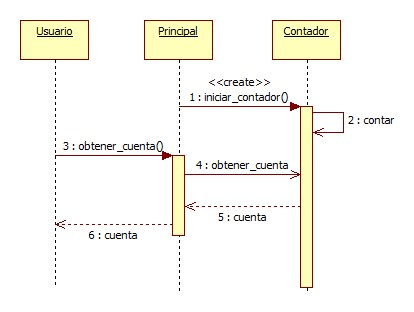
\includegraphics[width=0.50\textwidth, height = 7cm]{Secuencia2}
  \caption{Diagrama de secuencia del usuario obteniendo la cuenta de uno de los contadores}\label{fig:secuencia2}
\end{figure}


% \begin{figure}[H]
%   \centering
%   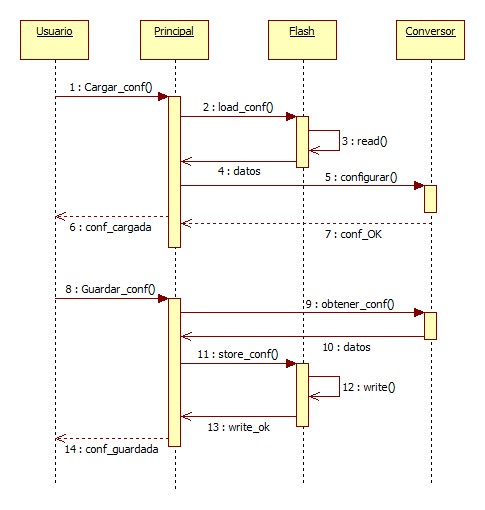
\includegraphics[width=0.60\textwidth, height = 8cm]{Secuencia3}
%   \caption{Diagrama de secuencia 3}\label{fig:secuencia3}
% \end{figure}

% subsubsection diagramas_de_secuencia (end)
% section diseno_del_software (end)

\clearpage
